\documentclass[../main]{subfiles}
\begin{document}

\chapter{HDB3 码型变换}%
\label{cha:hdb3}

% \section{实验目的}%
% \label{sec:\arabic{chapter}aim}
%
% \begin{itemize}
%   \item 了解几种常用的数字基带信号的特征和作用。
%   \item 掌握 HDB3 码的编译规则。
%   \item 了解滤波法位同步在的码型变换过程中的作用。
% \end{itemize}
%
% \section{实验器材}%
% \label{sec:\arabic{chapter}equipment}
%
% \begin{table}[htbp]
%   \centering
%   \caption{实验器材}%
%   \label{tab:\arabic{chapter}equipment}
%   \csvautobooktabular[respect percent]{tab/\arabic{chapter}equipment.csv}
% \end{table}
%
\section{实验原理}%
\label{sec:\arabic{chapter}principle}

\begin{figure}[htbp]
  \centering
  \includegraphics[
    width = 0.8\linewidth,
  ]{\arabic{chapter}dia}
  \caption{实验原理框图}%
  \label{fig:\arabic{chapter}dia}
\end{figure}

我们知道 AMI 编码规则是遇到 0 输出 0,遇到 1 则交替输出 +1 和 -1。而 HDB3 编
码由于需要插入破坏位 B,因此,在编码时需要缓存 3bit 的数据。当没有连续 4 个连
0 时与 AMI 编码规则相同。当 4 个连 0 时最后一个 0 变为传号 A,其极性与前一个
A 的极性相反。若该传号与前一个 1 的极性不同,则还要将这 4 个连 0 的第一个 0
变为 B,B 的极性与 A 相同。实验框图中编码过程是将信号源经程序处理后,得到
HDB3-A1 和 HDB3-B1 两路信号,再通过电平转换电路进行变换,从而得到 HDB3 编码
波形。

同样 AMI 译码只需将所有的 $\pm 1$ 变为 1,0 变为 0 即可。而 HDB3 译码只需找到
传号 A ,将传号和传号前 3 个数都清 0 即可。传号 A 的识别方法是:该符号的极性
与前一极性相同,该符号即为传号。实验框图中译码过程是将 HDB3 码信号送入到电平
逆变换电路,再通过译码处理,得到原始码元。

\section{实验步骤}%
\label{sec:\arabic{chapter}procedure}

\subsection{HDB3 编译码(256kHz 归零码实验)}%
\label{sub:rz}

% 本项目通过选择不同的数字信源,分别观测编码输入及时钟,译码输出及时钟,观察编
% 译码延时以及验证 HDB3 编译码规则。

% \begin{table}[htbp]
%   \centering
%   \caption{连线}%
%   \label{tab:\arabic{chapter}\arabic{subsection}}
%   \scriptsize
%   \csvautobooktabular[respect percent]{tab/\arabic{chapter}\arabic{subsection}.csv}
% \end{table}

% \begin{enumerate}
%   \item 关电,按表~\ref{tab:\arabic{chapter}\arabic{subsection}}所示进行连线。
%   \item 开电,设置主控菜单,选择【主菜单】→【通信原理】→【HDB3 编译码】 →【归
%     零码实验】。将模块 13 的开关 S3 分频设置拨为 0011,即提取 512K 同步时钟。
%   \item 此时系统初始状态为:编码输入信号为 256k 的 PN 序列。
%   \item 实验操作及波形观测。
\begin{enumerate}
  \item 用示波器分别观测编码输入的数据 TH3 和编码输出的数据 TH1 (HDB3 输
    出)图~\ref{fig:rz/hdb3_wave},观察记录波形,有数字示波器的可以观测编
    码输出信号频谱图~\ref{fig:rz/hdb3_spectrum}

    \begin{Exercise}[title = 思考]
      验证 HDB3 编码规则。
    \end{Exercise}

    \begin{Answer}
      HDB3 译码延迟5个码元周期。截取其中一部分见表~\ref{tab:hdb3},可见符合
      HDB3 编码规则。
    \end{Answer}

    \begin{table}[htbp]
      \centering
      \caption{HDB3}%
      \label{tab:hdb3}
      \csvautobooktabular[respect percent]{tab/hdb3.csv}
    \end{table}

    % 注:观察时注意码元的对应位置。
  \item 保持示波器测量编码输入数据 TH3 的通道不变,另一通道测量中间测试点
    TP2 (HDB3-A1),观察基带码元的变换波形图~\ref{fig:rz/a1_wave}。
  \item 保持示波器测量编码输入数据 TH3 的通道不变,另一通道测量中间测试点
    TP3 (HDB3-B1),观察基带码元的变换波形图~\ref{fig:rz/b1_wave}。
  \item 用示波器分别观测模块 8 的 TP2(HDB3-A1)和 TP3(HDB3-B1),可从频域角
    度观察信号所含 256kHz 频谱分量情况图~\ref{fig:rz/a1_spectrum}和
    图~\ref{fig:rz/b1_spectrum};或用示波器减法功能观察 HDB3-A1 与
    HDB3-B1 相减后的波形情况图~\ref{fig:rz/a1_b1_wave},并与 HDB3 编码输出波形
    图~\ref{fig:rz/hdb3_wave}相比较。
  \item 用示波器对比观测编码输入的数据和译码输出的数据,观察记录 HDB3 译
    码波形与输入信号波形图~\ref{fig:rz/codec}。

    \begin{Exercise}[title = 思考]
      译码过后的信号波形与输入信号波形相比延时多少?
    \end{Exercise}

    \begin{Answer}
      由图~\ref{fig:rz/codec}可以读出延时 0.04 ms。
    \end{Answer}

  \item 用示波器分别观测 TP4 (HDB3-A2)和 TP8 (HDB3-B2),从时域
    图~\ref{fig:rz2/a2_b2_wave}或频域角度图~\ref{fig:rz2/a2_spectrum}和
    图~\ref{fig:rz2/b2_spectrum}了解 HDB3 码经电平变换后的波形情况。
  \item 用示波器分别观测模块 8 的 TH7 (HDB3 输入)
    图~\ref{fig:rz/hdb3_wave}和 TH5 (单极性码)
    图~\ref{fig:rz2/single_wave},从频域角度观测双极性码
    图~\ref{fig:rz/hdb3_spectrum}和单极性码
    图~\ref{fig:rz2/single_spectrum}的 256kHz 频谱分量情况。
  \item 用示波器分别观测编码输入的时钟和译码输出的时钟
    图~\ref{fig:rz2/clock},观察比较恢复出的位时钟波形与原始位时钟
    信号的波形。
\end{enumerate}
% \end{enumerate}

\begin{figure}[htbp]
  \centering
  \begin{subfigure}[htbp]{0.45\linewidth}
    \centering
    \includegraphics[
      width = \linewidth,
    ]{rz/hdb3_wave}
    \caption{HDB3 波形}%
    \label{fig:rz/hdb3_wave}
  \end{subfigure}
  \quad
  \begin{subfigure}[htbp]{0.45\linewidth}
    \centering
    \includegraphics[
      width = \linewidth,
    ]{rz/hdb3_spectrum}
    \caption{HDB3 频谱}%
    \label{fig:rz/hdb3_spectrum}
  \end{subfigure}

  \begin{subfigure}[htbp]{0.45\linewidth}
    \centering
    \includegraphics[
      width = \linewidth,
    ]{rz/a1_wave}
    \caption{A1 波形}%
    \label{fig:rz/a1_wave}
  \end{subfigure}
  \quad
  \begin{subfigure}[htbp]{0.45\linewidth}
    \centering
    \includegraphics[
      width = \linewidth,
    ]{rz/b1_wave}
    \caption{B1 波形}%
    \label{fig:rz/b1_wave}
  \end{subfigure}

  \begin{subfigure}[htbp]{0.45\linewidth}
    \centering
    \includegraphics[
      width = \linewidth,
    ]{rz/a1_spectrum}
    \caption{A1 频谱}%
    \label{fig:rz/a1_spectrum}
  \end{subfigure}
  \quad
  \begin{subfigure}[htbp]{0.45\linewidth}
    \centering
    \includegraphics[
      width = \linewidth,
    ]{rz/b1_spectrum}
    \caption{B1 频谱}%
    \label{fig:rz/b1_spectrum}
  \end{subfigure}

  \begin{subfigure}[htbp]{0.45\linewidth}
    \centering
    \includegraphics[
      width = \linewidth,
    ]{rz/a1_b1_wave}
    \caption{A1 - B1 波形}%
    \label{fig:rz/a1_b1_wave}
  \end{subfigure}
  \quad
  \begin{subfigure}[htbp]{0.45\linewidth}
    \centering
    \includegraphics[
      width = \linewidth,
    ]{rz/codec}
    \caption{HDB3 译码输出}%
    \label{fig:rz/codec}
  \end{subfigure}
  \caption{归零}%
  \label{fig:rz}
\end{figure}

\begin{figure}[htbp]
  \centering
  \begin{subfigure}[htbp]{0.45\linewidth}
    \centering
    \includegraphics[
      width = \linewidth,
    ]{rz2/a2_b2_wave}
    \caption{A2 、 B2 波形}%
    \label{fig:rz2/a2_b2_wave}
  \end{subfigure}
  \quad
  \begin{subfigure}[htbp]{0.45\linewidth}
    \centering
    \includegraphics[
      width = \linewidth,
    ]{rz2/clock}
    \caption{编码输入时钟和译码输出时钟}%
    \label{fig:rz2/clock}
  \end{subfigure}

  \begin{subfigure}[htbp]{0.45\linewidth}
    \centering
    \includegraphics[
      width = \linewidth,
    ]{rz2/a2_spectrum}
    \caption{A2 频谱}%
    \label{fig:rz2/a2_spectrum}
  \end{subfigure}
  \quad
  \begin{subfigure}[htbp]{0.45\linewidth}
    \centering
    \includegraphics[
      width = \linewidth,
    ]{rz2/b2_spectrum}
    \caption{B2 频谱}%
    \label{fig:rz2/b2_spectrum}
  \end{subfigure}

  \begin{subfigure}[htbp]{0.45\linewidth}
    \centering
    \includegraphics[
      width = \linewidth,
    ]{rz2/single_wave}
    \caption{单极性波形}%
    \label{fig:rz2/single_wave}
  \end{subfigure}
  \quad
  \begin{subfigure}[htbp]{0.45\linewidth}
    \centering
    \includegraphics[
      width = \linewidth,
    ]{rz2/single_spectrum}
    \caption{单极性频谱}%
    \label{fig:rz2/single_spectrum}
  \end{subfigure}
  \caption{归零}%
  \label{fig:rz2}
\end{figure}

\begin{Exercise}[title = 思考]
  此处输入信号采用的单极性码,可较好的恢复出位时钟信号,如果输入信号采用的是
  双极性码,是否能观察到恢复的位时钟信号,为什么?
\end{Exercise}

\begin{Answer}
  不能,因为双极性码功率谱密度不含定时分量。
\end{Answer}

\begin{align}
  P_{1\mathrm{rz}}(f) = &
  \frac{T_\mathrm{s}}{16}{\left(\mathrm{sinc}\frac{fT_\mathrm{s}}{2}\right)}^2
  + \frac{1}{16} \sum^\infty_{n = -\infty} \delta(f -
  nf_\mathrm{s}){\left(\mathrm{sinc}\frac{fT_\mathrm{s}}{2}\right)}^2\\
  P_{2\mathrm{rz}}(f) = &
  \frac{T_\mathrm{s}}{4}{\left(\mathrm{sinc}\frac{fT_\mathrm{s}}{2}\right)}^2
\end{align}

\subsection{HDB3 编译码(256kHz 非归零码实验)}%
\label{sub:nrz}

% 本项目通过观测 HDB3 非归零码编译码相关测试点,了解 HDB3 编译码规则。

% \begin{enumerate}
%   \item 保持实验项目~\ref{sub:rz}的连线不变。
%   \item 开电,设置主控菜单,选择【主菜单】→【通信原理】→【HDB3 编译码】 →【非
%     归零码实验】。将模块 13 的开关 S3 分频设置拨为 0100,即提取 256K 同步时钟
%     。
%   \item 此时系统初始状态为:编码输入信号为 256K 的 PN 序列。
%   \item 实验操作及波形观测。

参照前面的 256kHz 归零码实验项目的步骤,进行相关测试。
结果见图~\ref{fig:nrz}和图~\ref{fig:nrz2}。不同之处在于非归零码不含定时分量。
% \end{enumerate}

\begin{figure}[htbp]
  \centering
  \begin{subfigure}[htbp]{0.45\linewidth}
    \centering
    \includegraphics[
      width = \linewidth,
    ]{nrz/hdb3_wave}
    \caption{HDB3 波形}%
    \label{fig:nrz/hdb3_wave}
  \end{subfigure}
  \quad
  \begin{subfigure}[htbp]{0.45\linewidth}
    \centering
    \includegraphics[
      width = \linewidth,
    ]{nrz/hdb3_spectrum}
    \caption{HDB3 频谱}%
    \label{fig:nrz/hdb3_spectrum}
  \end{subfigure}

  \begin{subfigure}[htbp]{0.45\linewidth}
    \centering
    \includegraphics[
      width = \linewidth,
    ]{nrz/a1_wave}
    \caption{A1 波形}%
    \label{fig:nrz/a1_wave}
  \end{subfigure}
  \quad
  \begin{subfigure}[htbp]{0.45\linewidth}
    \centering
    \includegraphics[
      width = \linewidth,
    ]{nrz/b1_wave}
    \caption{B1 波形}%
    \label{fig:nrz/b1_wave}
  \end{subfigure}

  \begin{subfigure}[htbp]{0.45\linewidth}
    \centering
    \includegraphics[
      width = \linewidth,
    ]{nrz/a1_spectrum}
    \caption{A1 频谱}%
    \label{fig:nrz/a1_spectrum}
  \end{subfigure}
  \quad
  \begin{subfigure}[htbp]{0.45\linewidth}
    \centering
    \includegraphics[
      width = \linewidth,
    ]{nrz/b1_spectrum}
    \caption{B1 频谱}%
    \label{fig:nrz/b1_spectrum}
  \end{subfigure}

  \begin{subfigure}[htbp]{0.45\linewidth}
    \centering
    \includegraphics[
      width = \linewidth,
    ]{nrz/a1_b1_wave}
    \caption{A1 - B1 波形}%
    \label{fig:nrz/a1_b1_wave}
  \end{subfigure}
  \quad
  \begin{subfigure}[htbp]{0.45\linewidth}
    \centering
    \includegraphics[
      width = \linewidth,
    ]{nrz/codec}
    \caption{HDB3 译码输出}%
    \label{fig:nrz/codec}
  \end{subfigure}
  \caption{非归零}%
  \label{fig:nrz}
\end{figure}

\begin{figure}[htbp]
  \centering
  \begin{subfigure}[htbp]{0.45\linewidth}
    \centering
    \includegraphics[
      width = \linewidth,
    ]{nrz2/a2_b2_wave}
    \caption{A2 、 B2 波形}%
    \label{fig:nrz2/a2_b2_wave}
  \end{subfigure}
  \quad
  \begin{subfigure}[htbp]{0.45\linewidth}
    \centering
    \includegraphics[
      width = \linewidth,
    ]{nrz2/clock}
    \caption{编码输入时钟和译码输出时钟}%
    \label{fig:nrz2/clock}
  \end{subfigure}

  \begin{subfigure}[htbp]{0.45\linewidth}
    \centering
    \includegraphics[
      width = \linewidth,
    ]{nrz2/a2_spectrum}
    \caption{A2 频谱}%
    \label{fig:nrz2/a2_spectrum}
  \end{subfigure}
  \quad
  \begin{subfigure}[htbp]{0.45\linewidth}
    \centering
    \includegraphics[
      width = \linewidth,
    ]{nrz2/b2_spectrum}
    \caption{B2 频谱}%
    \label{fig:nrz2/b2_spectrum}
  \end{subfigure}

  \begin{subfigure}[htbp]{0.45\linewidth}
    \centering
    \includegraphics[
      width = \linewidth,
    ]{nrz2/single_wave}
    \caption{单极性波形}%
    \label{fig:nrz2/single_wave}
  \end{subfigure}
  \quad
  \begin{subfigure}[htbp]{0.45\linewidth}
    \centering
    \includegraphics[
      width = \linewidth,
    ]{nrz2/single_spectrum}
    \caption{单极性频谱}%
    \label{fig:nrz2/single_spectrum}
  \end{subfigure}
  \caption{非归零}%
  \label{fig:nrz2}
\end{figure}

\subsection{HDB3 码对连 0 信号的编码、直流分量以及时钟信号提取观测}%
\label{sub:0_dc_clock}

% 本项目通过设置和改变输入信号的码型,观测 HDB3 归零码编码输出信号中对长连 0 码
% 信号的编码、含有的直流分量变化以及时钟信号提取情况,进一步了解 HDB3 码特性。

% \begin{table}[htbp]
%   \centering
%   \caption{连线}%
%   \label{tab:\arabic{chapter}\arabic{subsection}}
%   \scriptsize
%   \csvautobooktabular[respect percent]{tab/\arabic{chapter}\arabic{subsection}.csv}
% \end{table}

% \begin{enumerate}
%   \item 关电,按表~\ref{tab:\arabic{chapter}\arabic{subsection}}所示进行连线
%     。
%   \item 开电,设置主控菜单,选择【主菜单】→【通信原理】→【HDB3 编译码】 →【归
%     零码实验】。将模块 13 的开关 S3 分频设置拨为 0011,即提取 512K 同步时钟。
%     将模块 2 的开关 S1、S2、S3、S4 全部置为 11110000,使 DoutMUX 输出码型中含
%     有连 4 个 0 的码型状态。(或自行设置其他码值也可。)
%   \item 此时系统初始状态为:编码输入信号为 256kHz 的 32 位拨码信号。
%   \item 实验操作及波形观测。
\begin{enumerate}
  \item 观察含有长连 0 信号的 HDB3 编码波形。用示波器观测模块 8 的 TH3(编
    码输入-数据)和 TH1(HDB3 输出),观察信号中出现长连 0 时的波形变化情况
    图~\ref{fig:continue0}。

    % 注:观察时注意码元的对应位置。

    \begin{Exercise}[title = 思考]
      HDB3 编码与 AMI 编码波形有什么差别?
    \end{Exercise}

    \begin{Answer}
      HDB3 编码波形不含3个以上的连续0信号,AMI 编码波形可能含有,可利用这一特
      性进行宏观检错。编码方式上的差别见
      章节~\ref{sec:\arabic{chapter}principle},篇幅所限,不再赘述。
    \end{Answer}

  \item 观察 HDB3 编码信号中是否含有直流分量。将模块 2 的开关 S1、S2、S3
    、S4 拨为 00000000 00000000 00000000 00000011,用示波器分别观测编码输
    入数据和编码输出数据图~\ref{fig:dc/data},编码输入时钟和译码输出时钟
    图~\ref{fig:dc/clock},调节示波器,将信号耦合状况置为交流,观察记录波
    形图~\ref{fig:ac/data}和图~\ref{fig:ac/clock}。保持连线,拨码开关由 0
    到 1 逐位拨起,直到模块 2 的拨动开关置为 00111111 11111111 11111111
    11111111,

    \begin{Exercise}[title = 思考]
      观察拨码过程中编码输入数据和编码输出数据波形的变化情况。
    \end{Exercise}

    \begin{Answer}
      由图~\ref{fig:switch}可见,随着1 多 0 少,$\pm 1$出现越来越频繁。
    \end{Answer}

    \begin{Exercise}[title = 思考]
      HDB3 码是否存在直流分量?
    \end{Exercise}

    \begin{Answer}
      HDB3 码不存在直流分量。由直流耦合图~\ref{fig:dc}和交流耦合
      图~\ref{fig:ac},可以发现区别不大,从而佐证这一点。
    \end{Answer}

  \item 观察 HDB3 编码信号所含时钟频谱分量。将模块 2 的开关 S1、S2、S3、
    S4 全部置 0,用示波器先分别观测编码输入数据和编码输出数据
    图~\ref{fig:set0/data},再分别观测编码输入时钟和译码输出时钟
    图~\ref{fig:set0/clock},观察记录波形。再将模块 2 的开关 S1、S2 、S3、
    S4 全部置 1,观察记录波形图~\ref{fig:set1/data}和
    图~\ref{fig:set1/clock}。

    \begin{Exercise}[title = 思考]
      数据和时钟是否能恢复?注:有数字示波器的可以观测编码输出信号 FFT 频
      谱。在恢复时钟方面 HDB3 码与 AMI 码比较有哪一个更好?比较不同输入信
      号时两种码型的时钟恢复情况并联系其编码信号频谱分析原因。
    \end{Exercise}

    \begin{Answer}
      如图~\ref{fig:set0}和图~\ref{fig:set1},数据和时钟能恢复,在恢复时钟方
      面 HDB3 码比 AMI 码更好,因为如果输入信号出现连续多个 0, AMI 码的输出
      时钟信号会大大延迟,甚至无法恢复时钟信号。
    \end{Answer}
\end{enumerate}
% \end{enumerate}

\begin{figure}[htbp]
  \centering
  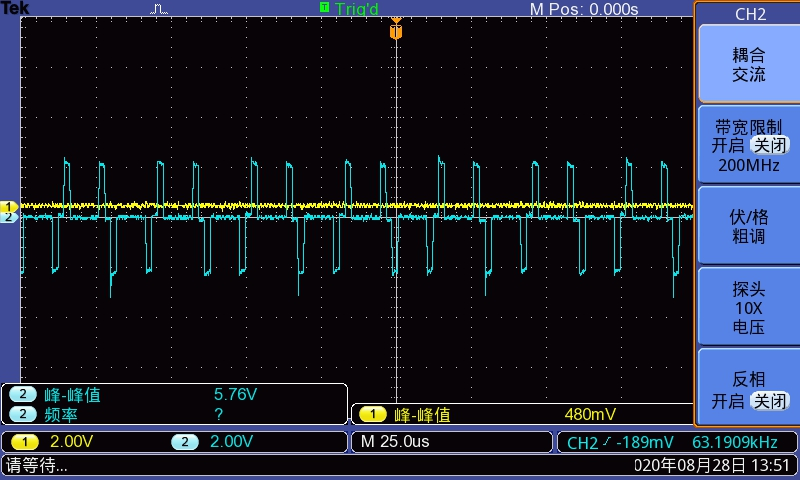
\includegraphics[
    width = 0.8\linewidth,
  ]{continue0}
  \caption{连续信号0}%
  \label{fig:continue0}
\end{figure}

\begin{figure}[htbp]
  \centering
  \begin{subfigure}[htbp]{0.45\linewidth}
    \centering
    \includegraphics[
      width = \linewidth,
    ]{dc/data}
    \caption{数据}%
    \label{fig:dc/data}
  \end{subfigure}
  \quad
  \begin{subfigure}[htbp]{0.45\linewidth}
    \centering
    \includegraphics[
      width = \linewidth,
    ]{dc/clock}
    \caption{时钟}%
    \label{fig:dc/clock}
  \end{subfigure}
  \caption{直流耦合}%
  \label{fig:dc}
\end{figure}

\begin{figure}[htbp]
  \centering
  \begin{subfigure}[htbp]{0.45\linewidth}
    \centering
    \includegraphics[
      width = \linewidth,
    ]{ac/data}
    \caption{数据}%
    \label{fig:ac/data}
  \end{subfigure}
  \quad
  \begin{subfigure}[htbp]{0.45\linewidth}
    \centering
    \includegraphics[
      width = \linewidth,
    ]{ac/clock}
    \caption{时钟}%
    \label{fig:ac/clock}
  \end{subfigure}
  \caption{交流耦合}%
  \label{fig:ac}
\end{figure}

\begin{figure}[htbp]
  \centering
  \begin{subfigure}[htbp]{0.45\linewidth}
    \centering
    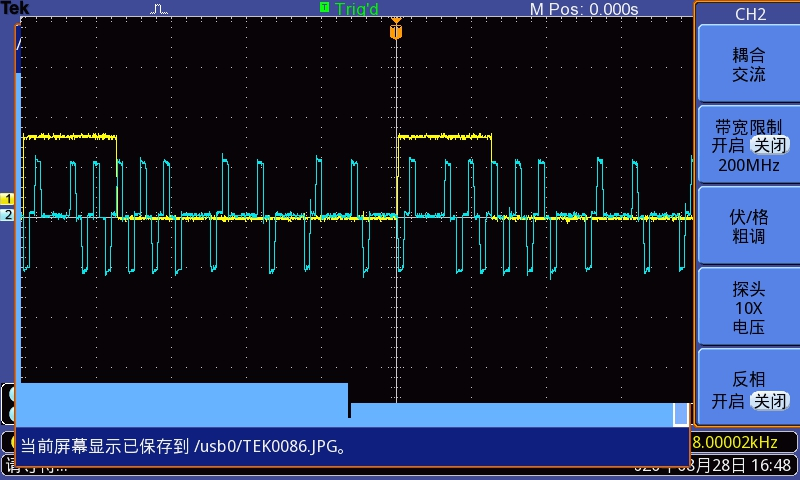
\includegraphics[
      width = \linewidth,
    ]{switch/1}
    \caption{拨动第1个字节}%
    \label{fig:switch/1}
  \end{subfigure}
  \quad
  \begin{subfigure}[htbp]{0.45\linewidth}
    \centering
    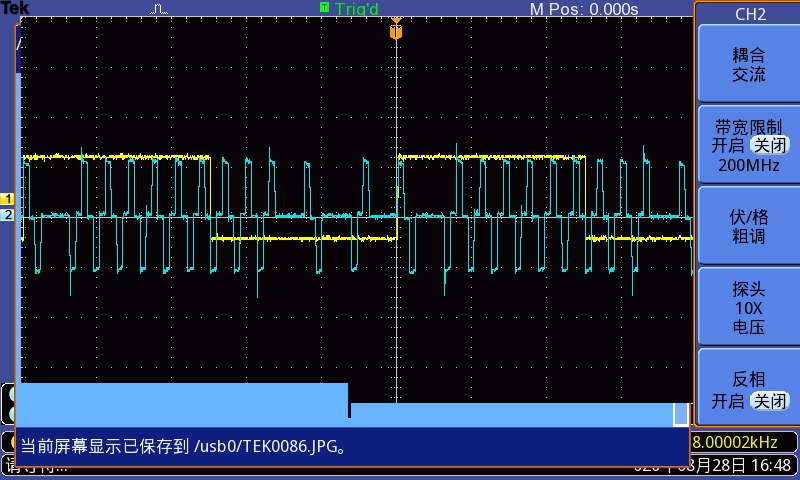
\includegraphics[
      width = \linewidth,
    ]{switch/2}
    \caption{拨动第2个字节}%
    \label{fig:switch/2}
  \end{subfigure}

  \begin{subfigure}[htbp]{0.45\linewidth}
    \centering
    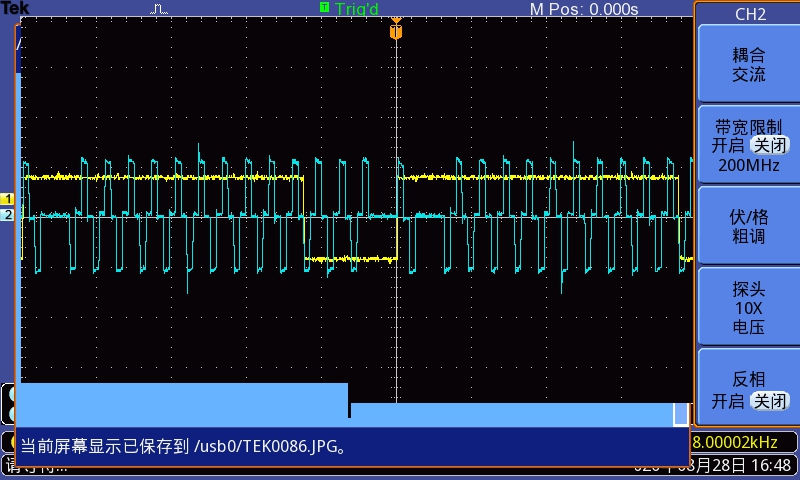
\includegraphics[
      width = \linewidth,
    ]{switch/3}
    \caption{拨动第3个字节}%
    \label{fig:switch/3}
  \end{subfigure}
  \quad
  \begin{subfigure}[htbp]{0.45\linewidth}
    \centering
    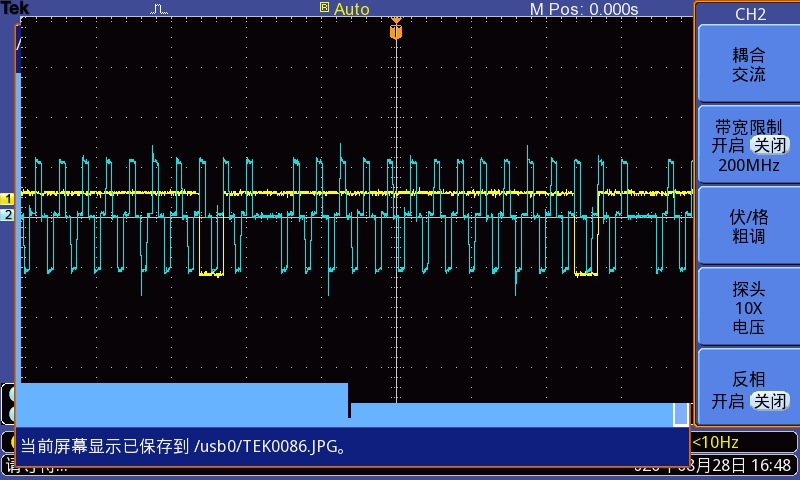
\includegraphics[
      width = \linewidth,
    ]{switch/4}
    \caption{拨动第4个字节}%
    \label{fig:switch/4}
  \end{subfigure}
  \caption{拨码开关}%
  \label{fig:switch}
\end{figure}

\begin{figure}[htbp]
  \centering
  \begin{subfigure}[htbp]{0.45\linewidth}
    \centering
    \includegraphics[
      width = \linewidth,
    ]{set0/data}
    \caption{数据}%
    \label{fig:set0/data}
  \end{subfigure}
  \quad
  \begin{subfigure}[htbp]{0.45\linewidth}
    \centering
    \includegraphics[
      width = \linewidth,
    ]{set0/clock}
    \caption{时钟}%
    \label{fig:set0/clock}
  \end{subfigure}
  \caption{清0}%
  \label{fig:set0}
\end{figure}

\begin{figure}[htbp]
  \centering
  \begin{subfigure}[htbp]{0.45\linewidth}
    \centering
    \includegraphics[
      width = \linewidth,
    ]{set1/data}
    \caption{数据}%
    \label{fig:set1/data}
  \end{subfigure}
  \quad
  \begin{subfigure}[htbp]{0.45\linewidth}
    \centering
    \includegraphics[
      width = \linewidth,
    ]{set1/clock}
    \caption{时钟}%
    \label{fig:set1/clock}
  \end{subfigure}
  \caption{置1}%
  \label{fig:set1}
\end{figure}

\section{实验报告}%
\label{sec:\arabic{chapter}report}

\begin{Exercise}
  分析实验电路的工作原理,叙述其工作过程。
\end{Exercise}

\begin{Answer}
  实验电路的工作原理见图~\ref{fig:\arabic{chapter}dia},工作过程见
  章节~\ref{sec:\arabic{chapter}principle}。
\end{Answer}

\begin{Exercise}
  根据实验测试记录,画出各测量点的波形图,并分析实验现象。
\end{Exercise}

\begin{Answer}
  HDB3 波形图见图~\ref{fig:rz/hdb3_wave}和图~\ref{fig:nrz/hdb3_wave},
  HDB3-A1 波形图见图~\ref{fig:rz/a1_wave}和图~\ref{fig:nrz/a1_wave},
  HDB3-B1 波形图见图~\ref{fig:rz/b1_wave}和图~\ref{fig:nrz/b1_wave},
  HDB3-A2 波形图和 HDB3-B2 波形图见图~\ref{fig:rz2/a2_b2_wave}和
  图~\ref{fig:nrz2/a2_b2_wave}, 。

  分析:数据和时钟先经过编码后得到 A1 和 B1,再经过变换得到 HDB3 码,HDB3 码
  经过反变换得到 A2 和 B2 再译码后得到时钟和数据。实验项目~\ref{sub:rz}和实验
  项目~\ref{sub:nrz}观察了归零和非归零情况下的波形。
  实验项目~\ref{sub:0_dc_clock}通过交流耦合后波形没有变化说明 HDB3 码没有直流
  分量。
\end{Answer}

\end{document}
